\chapter{Comparing current noise in biological and solid-state nanopores}
\label{chapter_3}

%% The following annotation is customary for chapter which have already been
%% published as a paper.
\blfootnote{This chapter has been published as: Alessio Fragasso, Sonja Schmid, Cees Dekker. "Comparing Current Noise in Biological and Solid-State Nanopores". ACS Nano 14(2), 1338–1349, (2020) \cite{Fragasso2020}.}

%% It is only necessary to list the authors if multiple people contributed
%% significantly to the chapter.
%\authors{Albert {\titleshape Einstein}}
%
%%% The '0pt' option ensures that no extra vertical space follows this epigraph,
%%% since there is another epigraph after it.
%\epigraph[0pt]{
%    Nature and nature's laws lay hid in the night; \\
%    God said `Let Newton be!' and all was light.
%}{Alexander Pope}
%
%\epigraph{
%    It did not last: the devil shouting `Ho. \\
%    Let Einstein be!' restore the status quo.
%}{Sir John Collings Squire}

\begin{abstract}
Nanopores bear great potential as single-molecule tools for bioanalytical sensing and sequencing, due to their exceptional sensing capabilities, high-throughput, and low cost. The detection principle relies on detecting small differences in the ionic current as biomolecules traverse the nanopore. A major bottleneck for the further progress of this technology is the noise that is present in the ionic current recordings, because it limits the signal-to-noise ratio and thereby the effective time resolution of the experiment. Here, we review the main types of noise at low and high frequencies and discuss the underlying physics. Moreover, we compare biological and solid-state nanopores in terms of the signal-to-noise ratio (SNR), the important figure of merit, by measuring translocations of a short ssDNA through a selected set of nanopores under typical experimental conditions. We find that SiN\textsubscript{x} solid-state nanopores provide the highest SNR, due to the large currents at which they can be operated and the relatively low noise at high frequencies. However, the real game-changer for many applications is a controlled slowdown of the translocation speed, which for MspA was shown to increase the SNR >160-fold. Finally, we discuss practical approaches for lowering the noise for optimal experimental performance and further development of the nanopore technology. 
\end{abstract}

%% Start the actual chapter on a new page.
\newpage


\section{Introduction}
%\pagestyle{myheadings}
%\markboth{\titlefont\titleshape\nouppercase{\leftmark}}{ciao}
Nanopores are promising tools for biosensing applications and sequencing of DNA and proteins, as they can resolve single analyte molecules, resolve structural modifications of molecules, and even discriminate between nucleotide sequences \cite{Dekker2007,Carson2015,Maglia2010,Feng2015a,Lin2018,Atas2012,Yang2018,Squires2013,Miles2012,Wu2014}. The detection mechanism is simple: while passing through the pore, a (part of a) molecule transiently blocks the ionic current, thereby inducing a small dip in the current signal, which is detectable by the electronics (Fig.\ref{fig:fig3.1}). The electrical read-out is carried out by an amplifier, which senses and amplifies the current signal, followed by a digitizer that performs the analog-to-digital conversion (ADC) of the data. Digital low-pass (LP) filtering is typically used to reduce the high-frequency noise, and thus improve the signal-to-noise ratio (SNR). Such a gain in SNR comes, however, at the expense of a lower time resolution, thereby imposing an inherent trade-off.


\begin{figure}[h]
	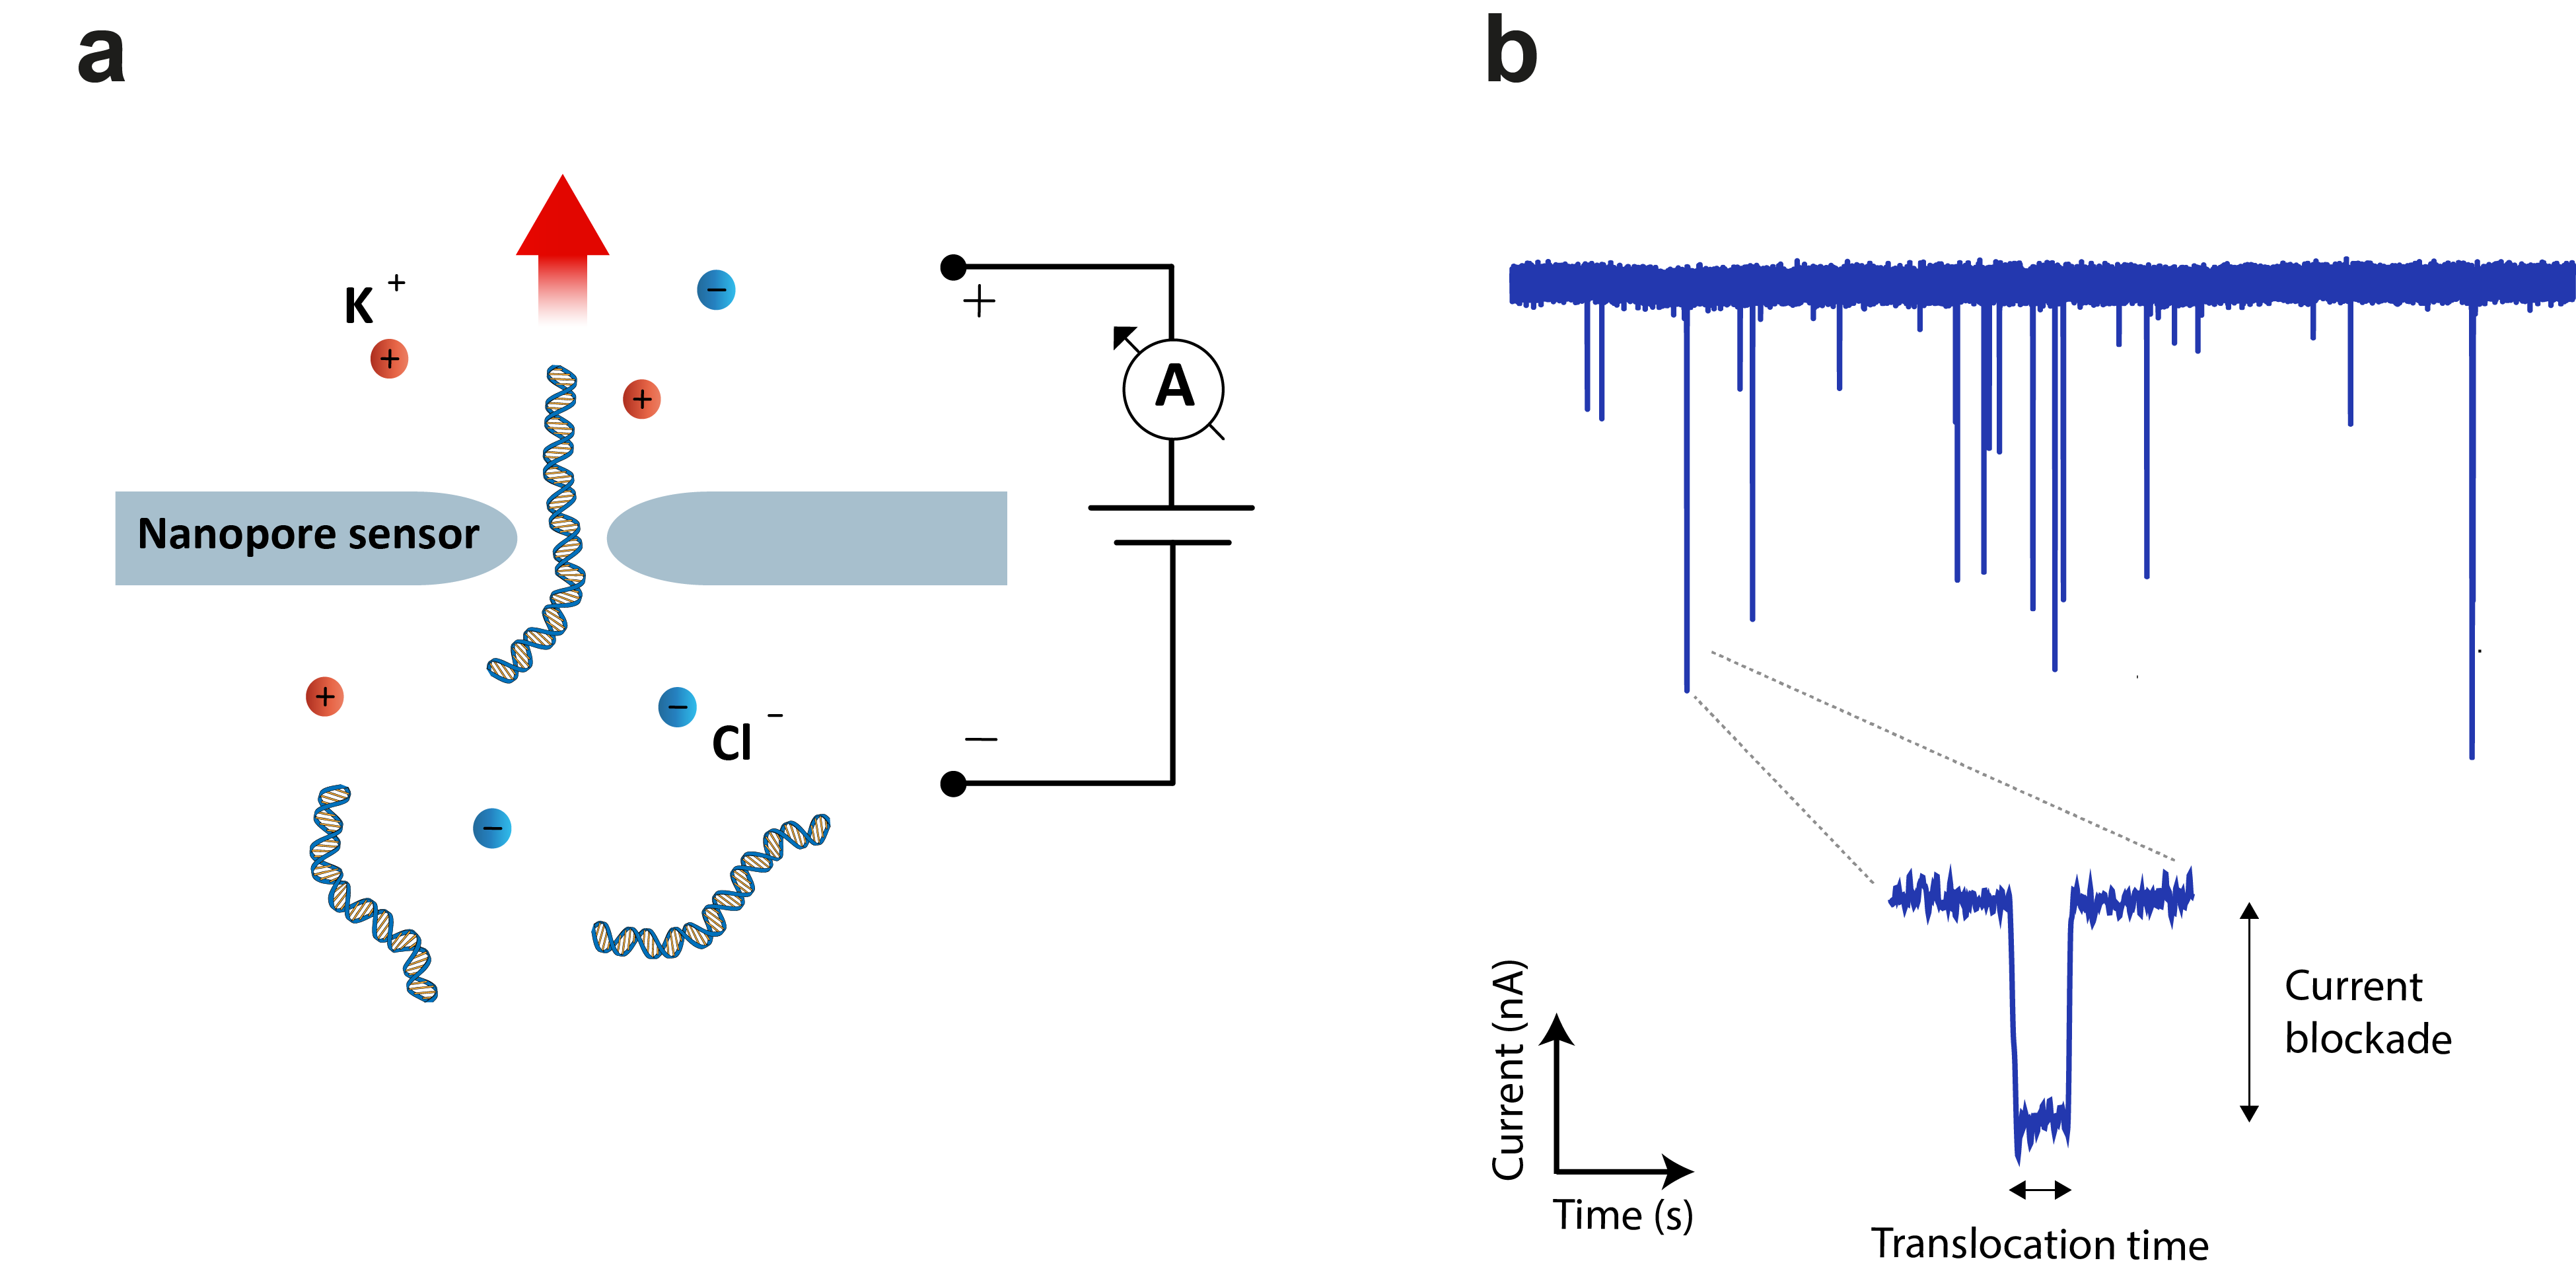
\includegraphics[width=\linewidth]{figures/Figure3.1.png}
     \caption{\textbf{Fundamental principle of nanopore sensing.} (a) A nanopore separates two aqueous compartments filled with electrolyte solution (\emph{e.g.} potassium chloride) and small molecules (\emph{e.g.} DNA) are electrokinetically pulled through the pore by an applied potential. (b) While passing through the nanopore, the molecule temporarily induces a partial current blockade which is detected by an amplifier. The signature of a single-molecule translocation event is generally characterized by the amplitude of the current blockade, which is proportional to the volume of the molecule in the nanopore, and by the dwell time, which depends on the electrophoretic driving force and transient interactions between the passing molecule and the pore surface.}
	\label{fig:fig3.1}
\end{figure}


 \noindent The detection of analytes with nanopores thus is, on the one hand, limited by the ionic current noise which requires LP filtering that sets a finite operating bandwidth \cite{Storm2005,Plesa2013}, but on the other hand, by the fast speed (typically sub-milliseconds) at which molecules translocate through the pore, which conversely requires a high time resolution for accurate sampling. Various approaches have been investigated in order to slow down the molecular translocation. For biological nanopores, a DNA-translocating motor protein (such as a helicase or polymerase) has been used to slowly feed a ssDNA strand into a protein pore for DNA sequencing \cite{Manrao2012,Derrington2010,Carter2018}. For solid-state nanopores fabricated in thin SiN\textsubscript{x} membranes \cite{Balan2014,Balan2015,Venta2013} or 2D materials (graphene \cite{Merchant2010,Schneider2010,Schneider2013}, boron nitride \cite{Zhou2013,Park2016,Liu2017}, molybdenum disulfide \cite{Graf2019,Liu2014,Feng2015}), various efforts have been made to either increase time resolution \cite{Balan2014,Balan2015,Rosenstein2012,Venta2013,Shekar2016,Thiel2019}, or slow down the translocation process \cite{Keyser2011} by the use of ionic liquids \cite{Feng2015}, pore surface engineering \cite{Wanunu2007} mechanical manipulation with a double pore system \cite{Pud2016}, optical trapping \cite{Gilboa2015}, and sequential DNA unzipping \cite{Yamazaki2018}. Nevertheless, while fingerprinting approaches have been developed to detect individual portions of a DNA sequence using dCas9 \cite{Yang2018,Weckman2019}, streptavidin \cite{Chen2017}, DNA hairpins \cite{Chen2019}, or DNA-origami as probes \cite{Bell2016}, the SNR has not yet allowed \emph{de novo} DNA sequencing with solid-state pores. An understanding of the noise sources that affect nanopore systems and how these govern the SNR is key for achieving signals wherein molecular structures can be resolved fast and reliably. Noise characteristics of nanopores have been reported in various isolated reports, but a systematic overview and comparison between biological and solid-state nanopores is lacking. 


In this review, we first describe the typical noise sources that affect the ionic current recordings of biological and solid-state nanopores, both at low and high frequencies. Next, we compare their respective performances of various nanopores using ssDNA poly(dT) translocations as a test system. We assess the SNR under typical experimental conditions for different protein pores \emph{Mycobacterium smegmatis} porin A (the M2 mutant with a neutral constriction and positively charged vestibule, subsequently referred to as MspA)\cite{Laszlo2016}, \emph{Staphylococcus aureus} alpha-hemolysin ($\alpha$-HL)\cite{Song1996,Menestrina1986}, \emph{Fragaceatoxin C} (the mutant of FraC with a positively charged constriction, referred to as ReFraC) \cite{Wloka2016,Huang2017a}, and SiN\textsubscript{x}\cite{Venta2013} and MoS\textsubscript{2}\cite{Graf2019} solid state nanopores. We find that biological pores generally exhibit lower noise (Fig.\ref{fig:fig3.2}a). Nevertheless, solid-state nanopores achieve the best SNR, largely because of the higher voltages and bandwidths that such devices can operate at, as compared to biological nanopores. Finally, we discuss approaches for lowering the ionic current noise and improving the SNR in biological and solid-state nanopores.


\section{Noise sources in nanopores}

Noise refers to any statistical fluctuation of a signal. It can be characterized by the standard deviation $\sigma$ or root-mean-square (rms) variation around the average value as measured over the full bandwidth $B$ of the signal, and by its power spectral density (PSD). Generally, noise is undesirable, as it can distort or even completely mask the actual signal. Nanopores typically operate by measuring a through-pore ionic current that is driven by a constant applied bias voltage. For the open-pore current measurement, where no analyte molecules are present, any deviation from the baseline current can be regarded as noise (Fig.\ref{fig:fig3.2}a).



\begin{figure}[!htb]
	\centering
	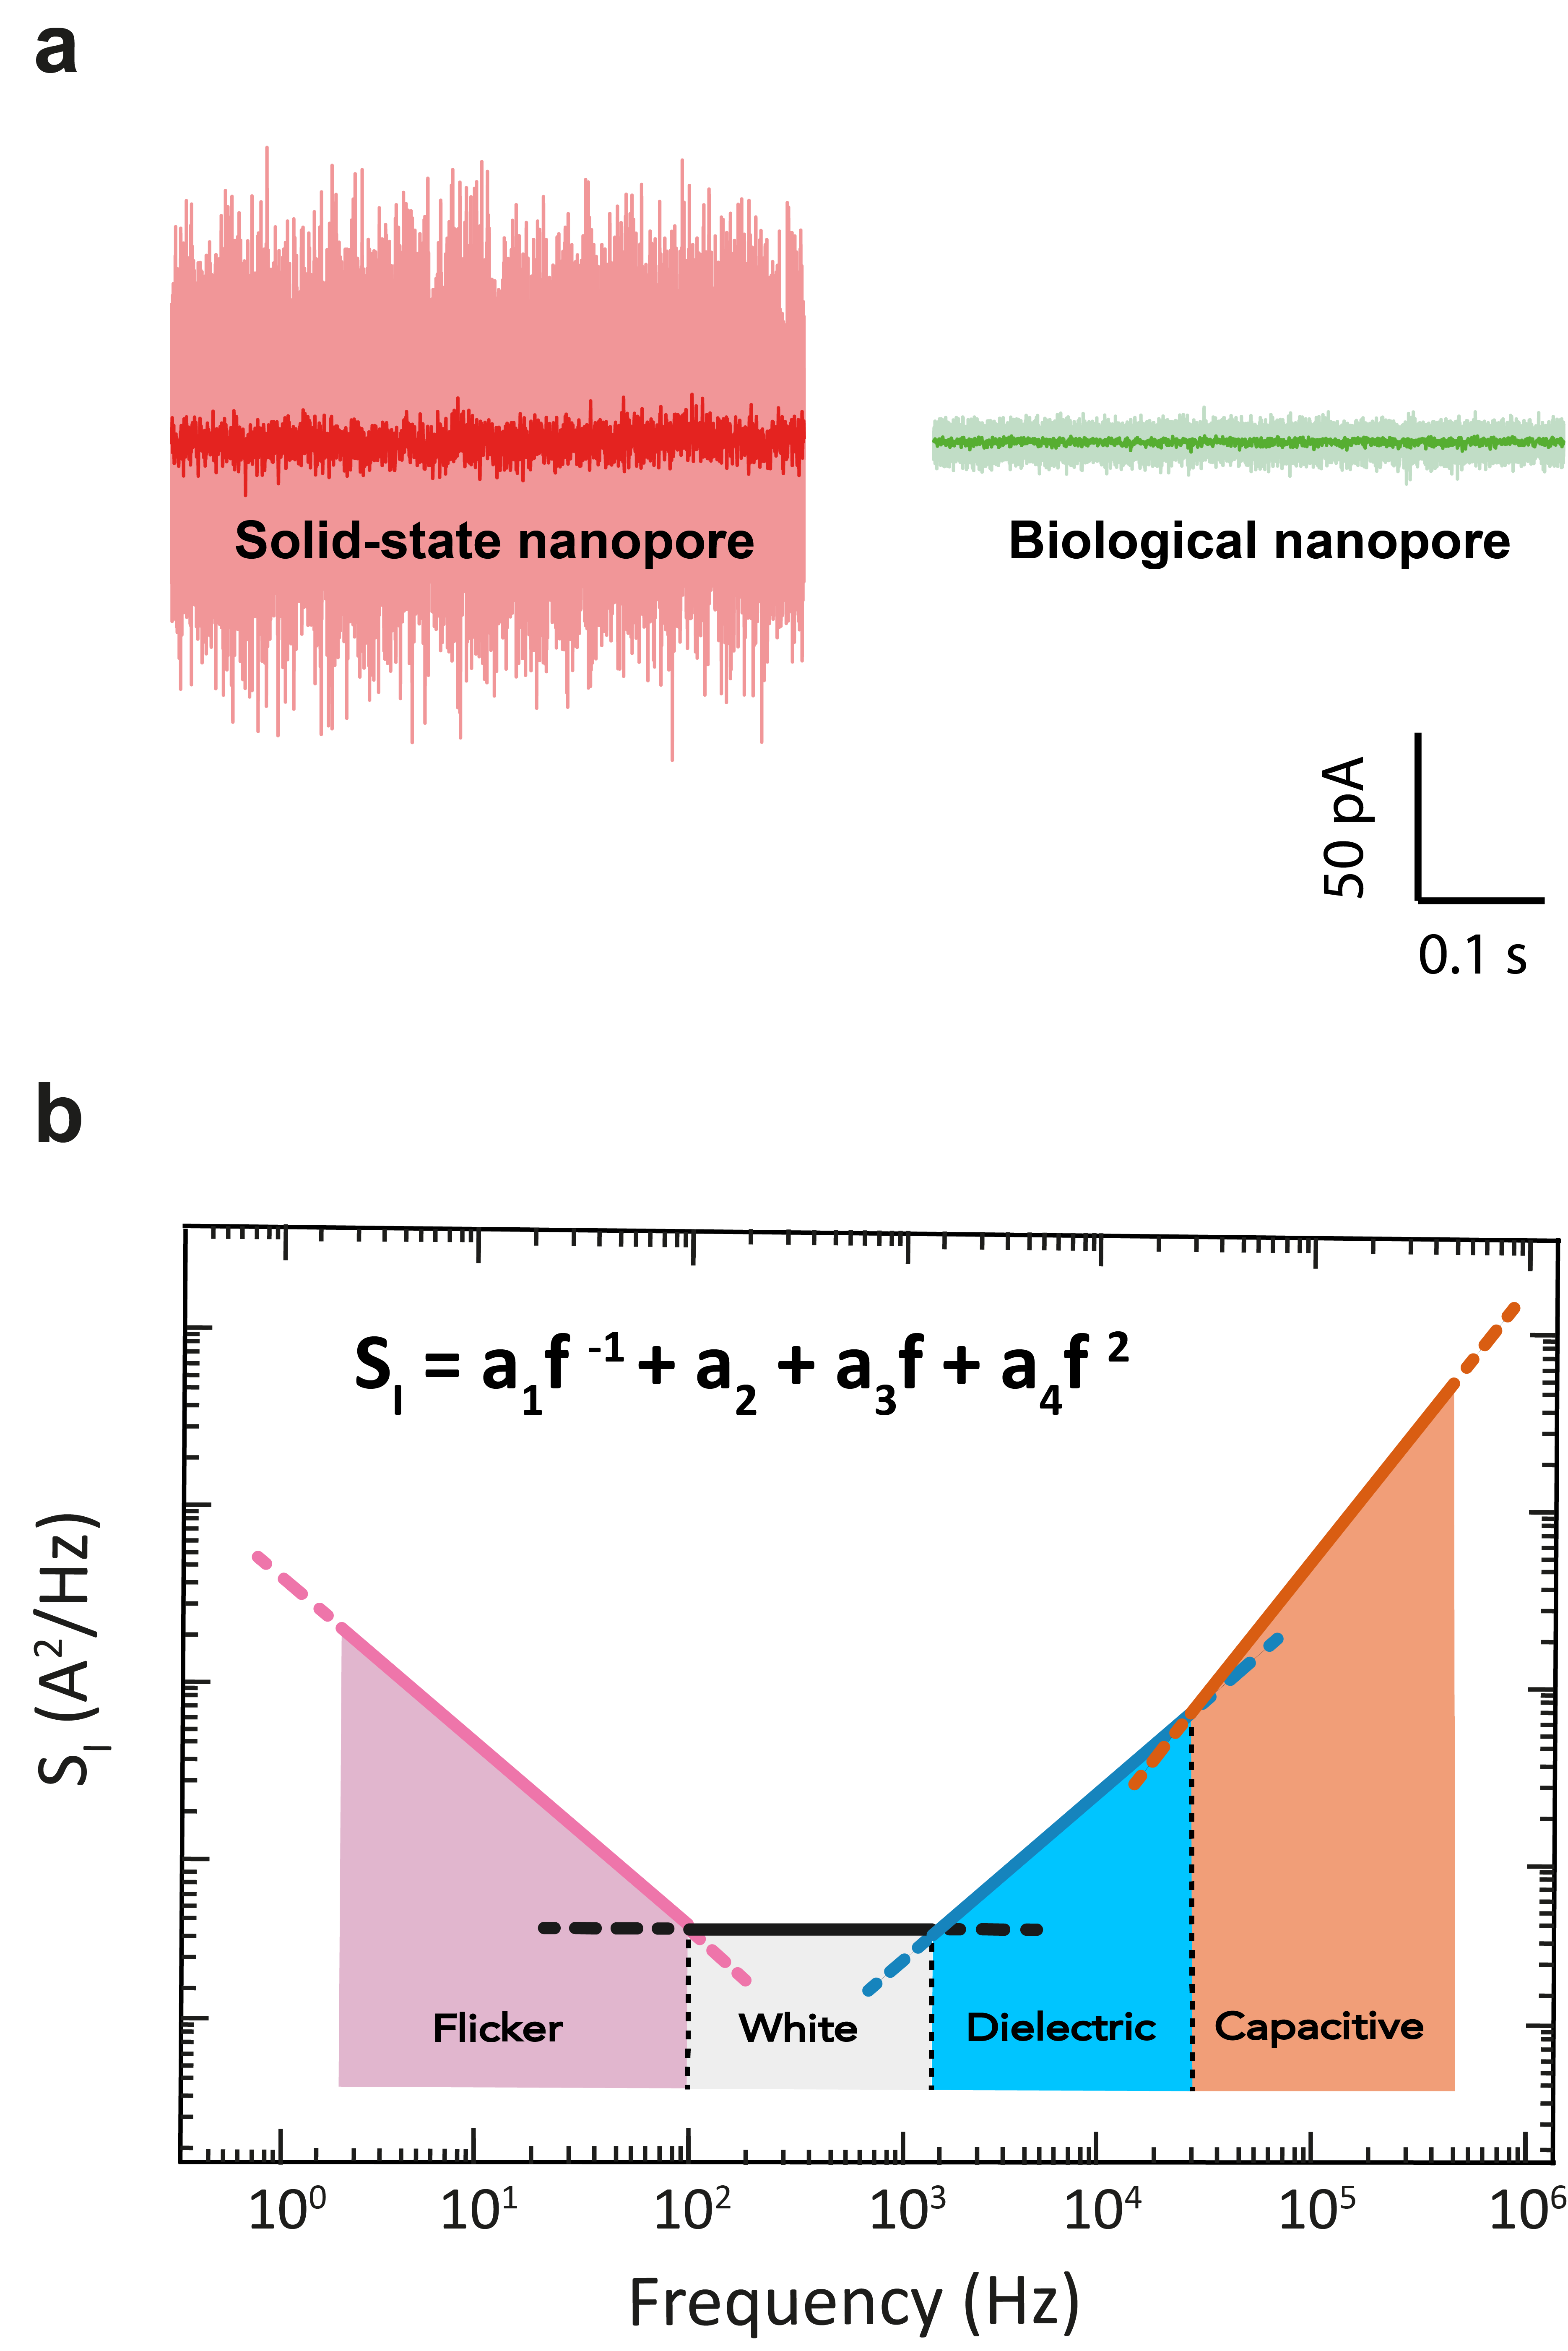
\includegraphics[width=0.6\linewidth]{figures/Figure3.2}
	 \caption{Ionic current noise in nanopores. (a) Example current traces for a 1.3 nm diameter solid-state SiN\textsubscript{x} nanopore (red) and a 1.4 nm diameter biological $\alpha$-HL pore (green), performed at a constant applied bias of 100 mV in 1 M KCl buffer at pH 7 at a bandwidth of 10 kHz (light) and 1 kHz (dark). $\alpha$-HL pore was measured using the typical Montal-Muller approach \cite{Montal1972}, with a bilayer diameter of $~$100 $\mu m$, as described by Maglia et al. (2010)\cite{Maglia2010}. The solid-state pore was fabricated on a Si-supported 20 nm-thick SiN\textsubscript{x} freestanding membrane using transmission electron microscopy. Currents through both pores were amplified with Axopatch 200B. (b) Schematic of the current Power Spectral Density (PSD) for a typical nanopore. Common types of noise are highlighted in the various frequency ranges.}
	\label{fig:fig3.2}
\end{figure}

Understanding the origins of noise is fundamental for optimizing signal detection. Nanopore systems exhibit a range of different noise sources \cite{Sakmann2009,Tabard-Cossa2013}. In Fig.\ref{fig:fig3.2}b, we illustrate the major current noise sources that affect nanopore systems at different frequencies. Generally, these can be divided in: (i) low-frequency ($\apprle$100 Hz) 1/f noise and protonation noise; (ii) shot noise and thermal current noise ($\sim$0.1-2 kHz), which are both white noise sources (i.e., frequency-independent); (iii) high-frequency dielectric ($\sim$1-10 kHz) and (iv) capacitive ($>$10 kHz) noise.  


In the low-frequency range, 1/f noise (also referred to as ‘flicker’ or ‘pink’ noise) typically is the dominant source of noise. Its power decreases with frequency $f$ following a 1/f\textsuperscript{$\beta$} scaling, with $\beta\approx 1$.  While this type of noise is found in many biological and physical systems, a fundamental understanding of it is still missing \cite{Milotti2002}. Based on phenomenological evidence, 1/f noise in nanopores has been associated with physical processes such as slow fluctuations in the number and mobility of the charge carriers \cite{Dutta1981,Zhang2018a,Jindal1981,Hooge1976}, nanometer-sized bubbles in the pore channel \cite{Smeets2006}, noise arising from the electrodes \cite{Wen2017}, mechanical fluctuations of the freestanding membrane (e.g. for 2D materials) \cite{Park2016,Heerema2015,Zhang2018}, and conformational changes in the case of biological nanopores \cite{Wohnsland1997,Bezrukov2000}. Smeets \emph{et al.} (2008) \cite{Smeets2008} found that Hooge’s phenomenological formula \cite{Hooge1976} could effectively describe the 1/f noise in solid-state \cite{Wen2017,Smeets2008,Smeets2009,Fragasso2019,Tasserit2010} nanopores, 



\begin{equation}\label{eqn:eq.3.1}
S_{I,1/f}=\frac{\alpha_H I^2}{N_c f^{\beta}},  
\end{equation}


\noindent where Hooge’s constant $\alpha_H$ is an empirical parameter that quantifies the magnitude of 1/f noise fluctuations, $I$ the ionic current, and $N_c$ the number of charge carriers in the pore volume, which was further validated by follow-up studies \cite{Wen2017,Smeets2009,Fragasso2019,Tasserit2010}. As discussed below, solid-state nanopores typically feature a relatively pronounced 1/f noise, whose microscopic origin often remains unresolved. For biological pores, the low-frequency noise is typically dominated by protonation noise, which is generated by protonation/de\-protonation of ionizable sites within the protein channel \cite{Nestorovich2003,Kasianowicz1993,Kasianowicz1995}. It  can be described by fluctuations between two different current levels with mean lifetimes $\tau_1$ and $\tau_2$ for the protonated and deprotonated states, respectively, yielding a Lorentzian-shaped component in the frequency spectrum (for a complete derivation see Machlup et al., 1954 \cite{Machlup1954}),


\begin{equation}\label{eqn:eq.3.2}
S_{I, protonation}=\frac{4(\Delta i)^2\tau^2}{\tau_1+\tau_2}\frac{1}{1+(2\pi f\tau)^2},
\end{equation}


\noindent where $\Delta i$ is the difference in current between the two levels, and $\tau$ is the characteristic relaxation time, that can be expressed as $\tau=(\tau_1\tau_2)/(\tau_1+\tau_2)$. For alpha-hemolysin, for example, $\tau$ was found to be $3.1\times 10^{-5}$ s\cite{Kasianowicz1995}. A distribution of multiple Lorentzian processes such as in Eq.\ref{eqn:eq.3.2} can lead to 1/f noise \cite{Dutta1981}. Temporal conformational changes of the pore channel can also generate conductance fluctuations resulting in 1/f noise. Such a phenomenon, also known as ‘channel breathing’, was reported to affect protein pores such as bacterial porin channels \cite{Wohnsland1997,Bezrukov2000}.

In the mid-frequency range (typically $\sim$0.1-2 kHz), a frequency-independent white noise is observed that derives from thermal noise (also known as Johnson-Nyquist noise) and shot noise. Thermal current noise is fundamental to any dissipative element \cite{Johnson1928,Nyquist1928} and adds to the current noise as


\begin{equation}\label{eqn:eq.3.3}
S_{I,thermal}=\frac{4k_BT}{R},
\end{equation}


\noindent where $k_B$ is the Boltzmann constant, $T$ is temperature, and $R$ the equivalent resistance of the nanopore. Shot noise, on the other hand, is due to the quantization of charge and is generated when charge carriers flow across a potential barrier \cite{Blanter2000,Schottky1918}. Its current-dependent contribution to the noise can be expressed as


\begin{equation}\label{eqn:eq.3.4}
S_{I,shot}=2Iq, 
\end{equation}

\noindent where $q$ is the charge of a single carrier. In practice, shot noise and thermal noise are comparable in magnitude for the conditions that are typically used in nanopore experiments. 


Another contribution to the nanopore noise originates from the loss conductance of the membrane and chip support \cite{Sakmann2009,Tabard-Cossa2013}. Such dissipation, resulting from dipolar relaxation and charge carrier migration (details can be found in Chen \emph{et al.}, 2014 \cite{Chen2004a}), generates thermal energy causing thermal noise, also known as dielectric noise \cite{Uram2008,Sherman-Gold2012}. As this loss conductance scales linearly with frequency, this noise can be described by


\begin{equation}\label{eqn:eq.3.5}
S_{I,dielectric}=8kT\pi C_{chip}Df,
\end{equation}

\noindent where $C_{chip}$ is the parasitic capacitance and $D$ a dissipation factor of the dielectric materials constituting the membrane and support chip. This source of noise typically dominates in the 2-10 kHz frequency range. To estimate $C_{chip}$, one can simply use the expression for a parallel plate capacitor $C=\epsilon A/d$, where $\epsilon$ is the dielectric constant of the membrane material and $A$ and $d$ are the area and the thickness of the membrane, respectively. For $f>10$ kHz, the current noise is determined by the input-referred thermal voltage noise $v_n$ across the total capacitance $C_{tot}$ at the amplifier input \cite{Sakmann2009,Tabard-Cossa2013},

\begin{equation}\label{eqn:eq.3.6}
S_{I,capacitance}=4\pi^2C_{tot}^2v_n^2f^2,
\end{equation}


\noindent where $v_n$ is the input voltage noise (3 nV/Hz\textsuperscript{-1}for the commonly used amplifier Axopatch 200B \cite{Sherman-Gold2012}, Molecular Devices, San Jose, USA). $C_{tot}$ is the total capacitance including the membrane and support chip capacitance $C_{chip}$, the capacitance $C_{amp}$ at the input of the amplifier, and the capacitance $C_w$ of the wiring between the electronics and the pore. Notably, $S_{I,capacitance}$ has an even stronger, $f^2$, frequency dependence than $S_{I,dielectric}$. The total current noise of a nanopore system over its full bandwidth is the sum of all contributions (Fig.\ref{fig:fig3.2}b), i.e., the sum of Eqs.\ref{eqn:eq.3.1}–\ref{eqn:eq.3.6}.  


\section{Noise in biological nanopores}

Biological nanopores are formed by the spontaneous insertion of membrane proteins into a lipid bilayer, which creates nanopores with typical diameters ranging from $\sim$1-4 nm \cite{Ayub2016}, although larger pores with diameters up to $\sim$40 nm, \emph{e.g.} the nuclear pore complex \cite{Yu2018}, are also found in nature. Figure \ref{fig:fig3.3}a shows a schematic of a standard setup for measuring the ionic current through such a protein pore. Briefly, a thick (tens of micrometers) insulating film of amorphous polytetrafluoro-ethylene (PTFE, or Teflon) separates two liquid compartments and contains a $\sim$50-100 $\mu$m sized hole where the lipid bilayer is assembled \cite{Maglia2010,Robertson2013}. Teflon is the preferred support material due to the relatively low high-frequency noise, and ease of fabrication \cite{Mayer2003}. Insertion of a protein pore (Fig.\ref{fig:fig3.3}b) short-circuits the insulating bilayer membrane and an ionic current between the two reservoirs can be measured by a pair of Ag/AgCl electrodes. The current signal is amplified by a transimpedance amplifier (e.g. Axopatch 200B) and digitized by an analog-to-digital converter (ADC, e.g. Axon Digidata, same supplier). To shield from external radiative electric noise, the flow-cell and the amplifier headstage are enclosed in a metallic Faraday cage \cite{Maglia2010}. For biological nanopores, ionic conductances are typically on the order of 0.1-2 nS.


Characteristic examples of the current PSD for 3 biological nanopores ($\alpha$-HL \cite{Song1996}, MspA, and ReFraC \cite{Wloka2016}) are shown in Figure \ref{fig:fig3.3}c, as measured at 1 M KCl, pH 7.5, under 50 mV applied bias. Noticeably, both $\alpha$-HL and MspA exhibit a noise plateau at low frequencies ($< 1$ kHz) which is due to protonation noise, cf. Eq.\ref{eqn:eq.3.2} for $f\ll 1/\tau$. The associated PSD is $\sim10{-4}$ to $10{-3}$ pA\textsuperscript{2}/Hz, which is higher than the corresponding white noise of $\sim 10{-5}$ pA\textsuperscript{2}/Hz, set by the sum of thermal and shot noise, Eq.\ref{eqn:eq.3.3} and \ref{eqn:eq.3.4}. In the context of single-molecule sensing, protonation noise in biological nanopores was first investigated by Bezrukov and Kasianowicz in the mid 1990s \cite{Kasianowicz1993,Kasianowicz1995}.


\begin{figure}[H]
	\centering
	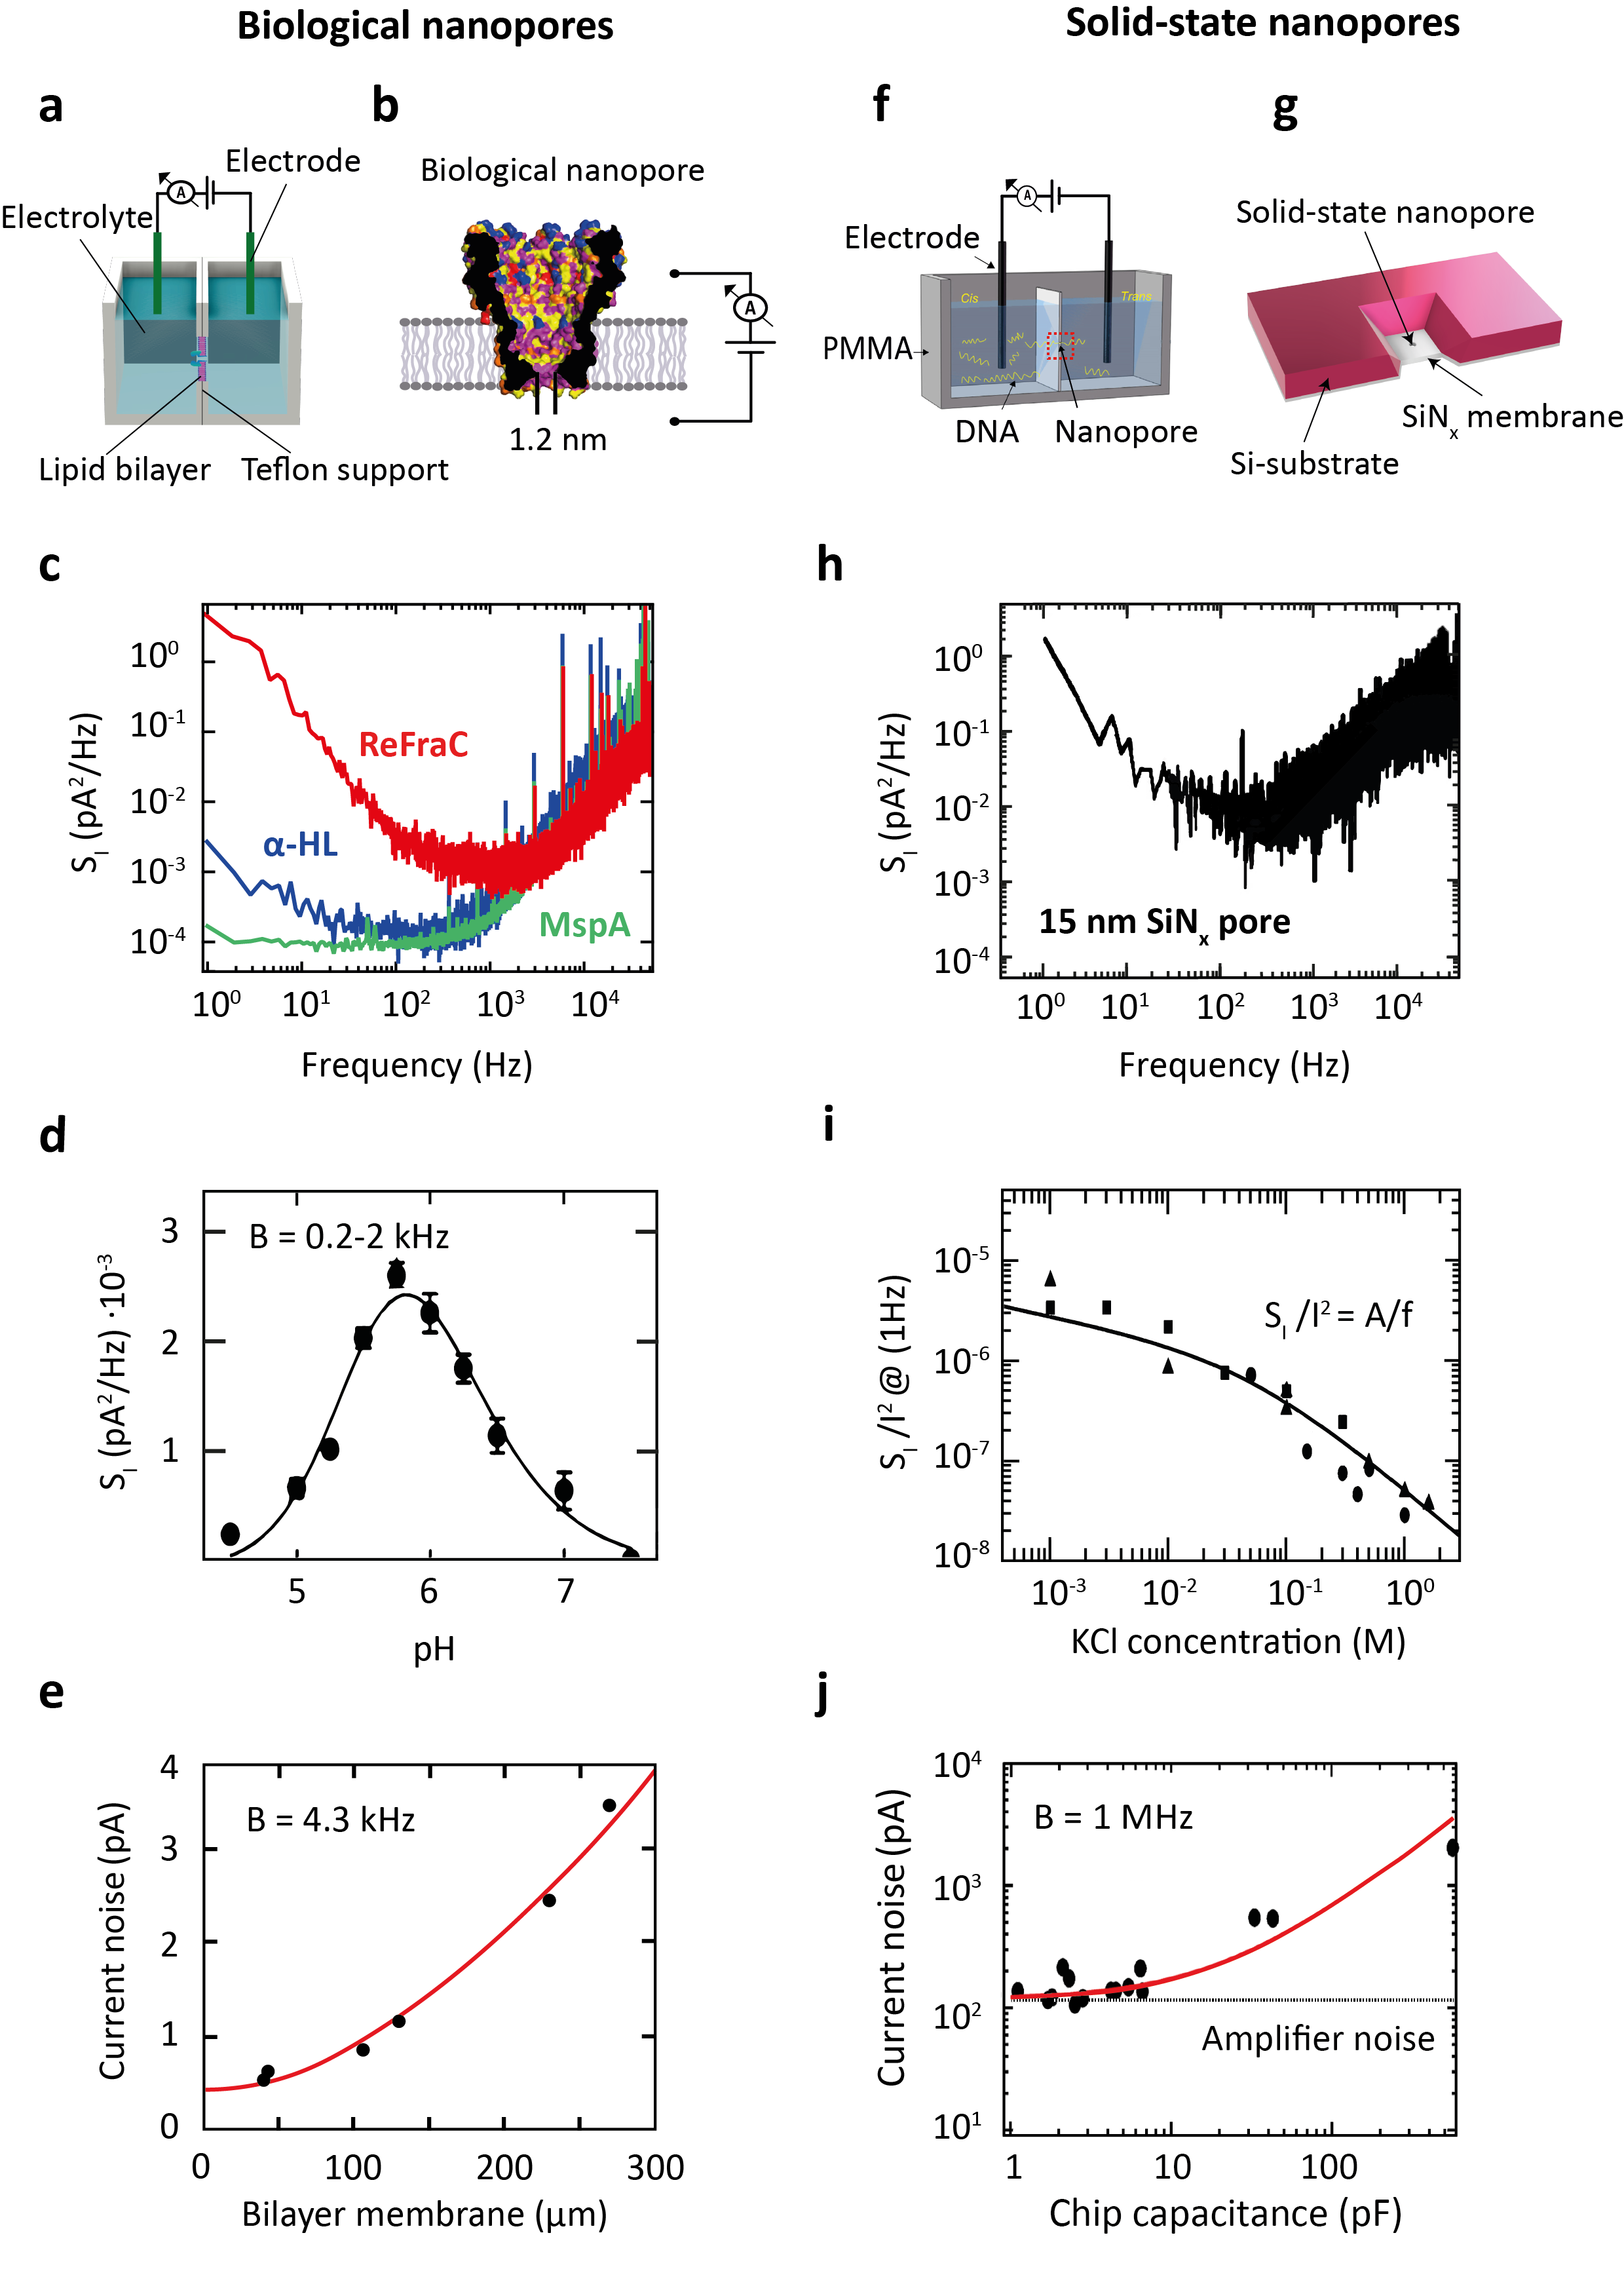
\includegraphics[width=0.8\linewidth]{figures/Figure3.3}
	\caption{Noise in biological and solid-state nanopores.
		(a) Standard setup used for measuring the ionic current through a biological nanopore embedded within a lipid membrane. (b) Sketch of a biological MspA nanopore \cite{Derrington2010}. Adapted with permission from Derrington, I. M. \emph{et al.}, 2010; 
		%Butler, T. Z.; Collins, M. D.; Manrao, E.; Pavlenok, M.; Niederweis, M.; Gundlach, J. H. Nanopore DNA Sequencing with MspA, Proc. Natl. Acad. Sci. 2010, 107, 16060–16065. Copyright \copyright 2010 National Academy of Sciences, U.S.A. 
		(c) Typical current PSD for three biological nanopores, ReFraC (D10R/K159E mutant of FraC)\cite{Wloka2016} (red), $\alpha$-HL (blue), and the D90N/D91N/D93N/D118R/E139K/D134R mutant of MspA (green), measured in the same setup at 50 mV applied voltage, 1 M KCl salt, pH 7. (d) Low-frequency protonation noise of $\alpha$-HL as a function of pH.67 Adapted with permission from Kasianowicz, J. J. \emph{et al.} 1995.
		%; Bezrukov, S. M. Protonation Dynamics of the Alpha-Toxin Ion Channel from Spectral Analysis of pH-Dependent Current Fluctuations, Biophys. J. 1995, 69, 94–105. Copyright \copyright 1995 The Biophysical Society. 
		(e)  Current noise I\textsubscript{rms} measured at a 4.3 kHz bandwidth of a lipid bilayer setup (where no pore was inserted) \emph{vs} the size of the bilayer membrane \cite{Mayer2003}. Adapted with permission from Mayer, M. \emph{et al.}, 2003
		%; Kriebel, J. K.; Tosteson, M. T.; Whitesides, G. M. Microfabricated Teflon Membranes for Low-Noise Recordings of Ion Channels in Planar Lipid Bilayers. Biophys. J. 2003, 85, 2684–2695. Copyright \copyright 2003 The Biophysical Society. 
		(f) Schematic of a typical flow cell for measuring the ionic current through a solid-state nanopore \cite{Feng2015a}. Adapted with permission from Feng, Y. \emph{et al.}, 2015.
		%; Zhang, Y.; Ying, C.; Wang, D.; Du, C. Nanopore-Based Fourth-Generation DNA Sequencing Technology. Genomics, Proteomics Bioinformatics 2015, 13, 4–16. Copyright \copyright 2015 The Authors. 
		(g) Sketch of a solid-state nanopore fabricated onto a Si-supported SiN\textsubscript{x} membrane. (h) Current PSD for a 15.6 nm SiN\textsubscript{x} solid-state nanopore. Data were measured at 100 mV applied voltage for 1 M KCl salt \cite{Smeets2008}. 
		(i) Relative low-frequency noise S\textsubscript{I}/I\textsuperscript{2} at 1 Hz versus salt concentration \cite{Smeets2008}. Solid line shows a fit to the data using Hooge’s relation, cf. Eq.\ref{eqn:eq.3.1}. (h) and (i) were adapted with permission from Smeets, R. M. M. \emph{et al.}, 2008.
		%; Keyser, U. F.; Dekker, N. H.; Dekker, C. Noise in Solid-State Nanopores, Proc. Natl. Acad. Sci. 2008, 105, 417–421. Copyright \copyright 2008 National Academy of Sciences, U.S.A. 
		(j) Current noise I\textsubscript{rms} measured at a 1 MHz bandwidth vs capacitance of the nanopore chip\cite{Balan2014}. Adapted with permission from Balan, A. \emph{et al.}, 2014.
		%; Machielse, B.; Niedzwiecki, D.; Lin, J.; Ong, P.; Engelke, R.; Shepard, K. L.; Drndić, M. Improving Signal-to-Noise Performance for DNA Translocation in Solid-State Nanopores at MHz Bandwidths. Nano Lett. 2014, 14, 7215–7220. Copyright \copyright 2014 American Chemical Society.
	}
	\label{fig:fig3.3}
\end{figure}



 Spectral analysis of the current noise of alpha-hemolysin pores revealed the presence of a Lorentzian-shaped component at low-frequencies ($0.2$–$2$ kHz). Given the strong dependence on pH (Fig.\ref{fig:fig3.3}d), this noise source was associated to the reversible protonation of ionizable residues occurring in the alpha-hemolysin constriction. This notion was further established in a later work by Nestorovich \emph{et al.} \cite{Nestorovich2003}, where the bacterial porin, OmpF, was shown to produce a similar pH-dependence of the protonation noise. 





\noindent ReFraC instead shows a pronounced 1/f noise with a PSD of $\sim$10{-1} pA\textsuperscript{2}/Hz at 1 Hz, which is almost three times more than for $\alpha$-HL and MspA. 1/f noise in biological nanopores was first studied by Benz and coworkers \cite{Wohnsland1997,Nekolla1994}, and described using Hooge’s model, Eq.\ref{eqn:eq.3.1}. The low-frequency fluctuations observed in a family of bacterial porins were associated with a number of possible phenomena, \emph{e.g.} gating of the pore channel\cite{Wohnsland1997}. In later work by Bezrukov and Winterhalter \cite{Bezrukov2000}, conformational changes of the protein pore channel, termed ‘channel breathing’ \cite{Lauger1985}, were discussed as the main cause for the observed 1/f noise.


At higher frequencies ($>1$ kHz), the noise in biological nanopores is dominated by dielectric noise arising from the loss conductance of the lipid membrane. In fact, since the dielectric loss and dielectric constant of the teflon are relatively low ($D=(0.8-2)\times 10^{-4}$ and $\epsilon_r=1.89-1.93$, respectively), the major contribution to the dielectric noise is set by the capacitance of the thin lipid bilayer membrane. This can be attenuated by reducing the area of the teflon hole (Fig.\ref{fig:fig3.3}e) \cite{Mayer2003,Akeson2009}. A noise characterization at even higher frequencies (MHz-GHz; above the experimentally accessible frequency range) was performed using molecular dynamics simulations based on a comprehensive model of MspA \cite{Bhattacharya2016}.

\section{Noise in solid-state nanopores}

Solid-state nanopores are generally fabricated in a freestanding membrane of a solid-state material such as silicon nitride (SiN\textsubscript{x}) \cite{Gibb2013}, graphene \cite{Merchant2010}, hexagonal boron nitride (h-BN) \cite{Gilbert2017}, or molybdenum disulfide (MoS\textsubscript{2}) \cite{Graf2019}, with thicknesses ranging from $\sim$0.3-30 nm. In common nanopore chips (Fig.\ref{fig:fig3.3}g), such a membrane is structurally supported by a $\sim$200-500 $\mu$m thick substrate material, typically silicon (Si) \cite{Gibb2013}, glass (SiO\textsubscript{2}) \cite{Balan2014}, or Pyrex \cite{Lee2014,Pitchford2015}. Nanopores can be drilled into the membrane in a variety of ways, e.g. by using a transmission electron microscope (TEM) \cite{Storm2003,VanDenHout2010}, focused ion beam milling (FIB) \cite{Lanyon2007,Schiedt2010}, reactive ion etching (RIE) ]\cite{Verschueren2018}], laser-etching \cite{Gilboa2019,Gilboa2018}, or by dielectric breakdown \cite{Pud2015,Kwok2014}, resulting in pore diameters from sub-1 nm to tens of nanometers. In a standard solid-state-nanopore experiment, the chip is sandwiched between two rubber O-rings that seal two compartments containing the electrolyte solution (Fig.\ref{fig:fig3.3}f). Alternatively, solid-state pores of $\sim$5-50 nm size can be made by mechanical pulling of hollow glass (SiO\textsubscript{2}) pipettes \cite{Piper2006,Xu2017,Bafna2016}, which are immersed in electrolyte during the measurement. Current sensing, amplification, and recording is the same as for biological nanopores. 




Figure \ref{fig:fig3.3}h displays a typical current PSD measured for a 15 nm diameter SiN\textsubscript{x} solid-state nanopore \cite{Smeets2008} in a 20 nm thick membrane. Characteristic of solid-state nanopores is the pronounced 1/f noise that dominates the low-frequency part of the spectrum ($<100$ Hz). It can originate from a range of physical processes, see Eq.\ref{eqn:eq.3.1} and associated discussion. Smeets \emph{et al.} 2006 \cite{Smeets2006} showed that poor wettability of the pore surface, associated with the formation of nanobubbles, resulted in high 1/f noise in SiN\textsubscript{x}. Tabard-Cossa \emph{et al.} \cite{Tabard-Cossa2007} discussed that high 1/f noise in SiN\textsubscript{x} pores correlates with surface contamination: inhomogeneities of the pore surface resulted in fluctuations of the number and mobility of charge carriers due to trapping at the pore surface \cite{Fragasso2019,Tabard-Cossa2007}, analogous to 1/f noise found in semiconductors \cite{Vandamme1994}. As shown by Smeets \emph{et al.} \cite{Smeets2008,Smeets2009}, such low-frequency noise in SiN\textsubscript{x} pores obeys Hooge’s relation, Eq.\ref{eqn:eq.3.1}, which describes an inverse proportionality between the 1/f current noise power and the number of charge carriers present within the nanopore volume (Fig.\ref{fig:fig3.3}i) \cite{Hooge1976}. For nanopores made in 2D materials, the 1/f noise depends strongly on the size of the freestanding area \cite{Zhou2013,Heerema2015,Zhang2018,Garaj2013}, indicating that mechanical fluctuations of the ultrathin 2D membrane (thickness $<1$ nm) are the main source. The high-frequency noise in solid-state nanopores is dominated by dielectric ($\sim$2-10 kHz) and capacitive noise ($>10$ kHz) \cite{Balan2014,Roelen2018}, see Fig.\ref{fig:fig3.3}j. The PSD of these noise sources depends mostly on the capacitance of the chip, cf. Eq.\ref{eqn:eq.3.5} and \ref{eqn:eq.3.6}, which in turn is set by the membrane and substrate size, thickness, and dielectric constant. Additionally, parasitic capacitances from the amplifier and the interconnects between nanopore and amplifier contribute to the total capacitance at the amplifier input.


\section{Comparing the performance of biological and so\-lid-state nanopores}

So far, we provided a general overview of the typical noise sources in biological and solid-state nanopores. We now turn to a mutual comparison between these two classes of nanopores. We compare their performances in terms of the SNR – a more relevant figure of merit than the mere magnitude of the current noise. We define the SNR as the ratio between the signal modulation $\Delta$I produced by the translocation of a ssDNA molecule, and the baseline current rms (I\textsubscript{rms}) measured at the operating bandwidth (Fig.\ref{fig:fig3.4}a). Although other definitions of SNR are found in the literature, \emph{e.g.} as the ratio between open pore current and baseline current noise I\textsubscript{o}/I\textsubscript{rms} \cite{Rosenstein2013} or the capability to discern current levels when sequencing DNA \cite{Manrao2012,Laszlo2016}, we find this definition the most appropriate for the diverse nanopore systems compared in our study.

Given that the experimental conditions reported in the literature differ considerably, we carried out a dedicated comparative study by complementing reported data with new data that were, to the extent possible, obtained in our lab under the same experimental conditions. The bandwidth was chosen such as to fully resolve the current blockade $\Delta$I generated by the poly(dT) substrate (avoiding a reduced $\Delta$I due to a too narrow bandwidth). The translocation time in turn, is determined by a combination of electrophoresis, electro-osmosis, and interactions between the passing molecule and the pore surface, which will depend on each individual nanopore system. The applied bias was chosen as to maximize the current signal and is limited by experimental conditions, as will be discussed below. We selected 5 popular nanopore systems, MspA , $\alpha$-HL, ReFraC, MoS\textsubscript{2}, and SiN\textsubscript{x}, that are commonly used and that were shown to possess good spatiotemporal resolution, allowing for accurate discrimination of short homopolymers \cite{Manrao2012,Feng2015,Venta2013,Wloka2016,Manrao2010}. All pores considered had a similar diameter of $\sim$1.3 nm. Figure \ref{fig:fig3.4}b illustrates the relative sizes of the different pores.

\begin{figure}[H]
	\centering
	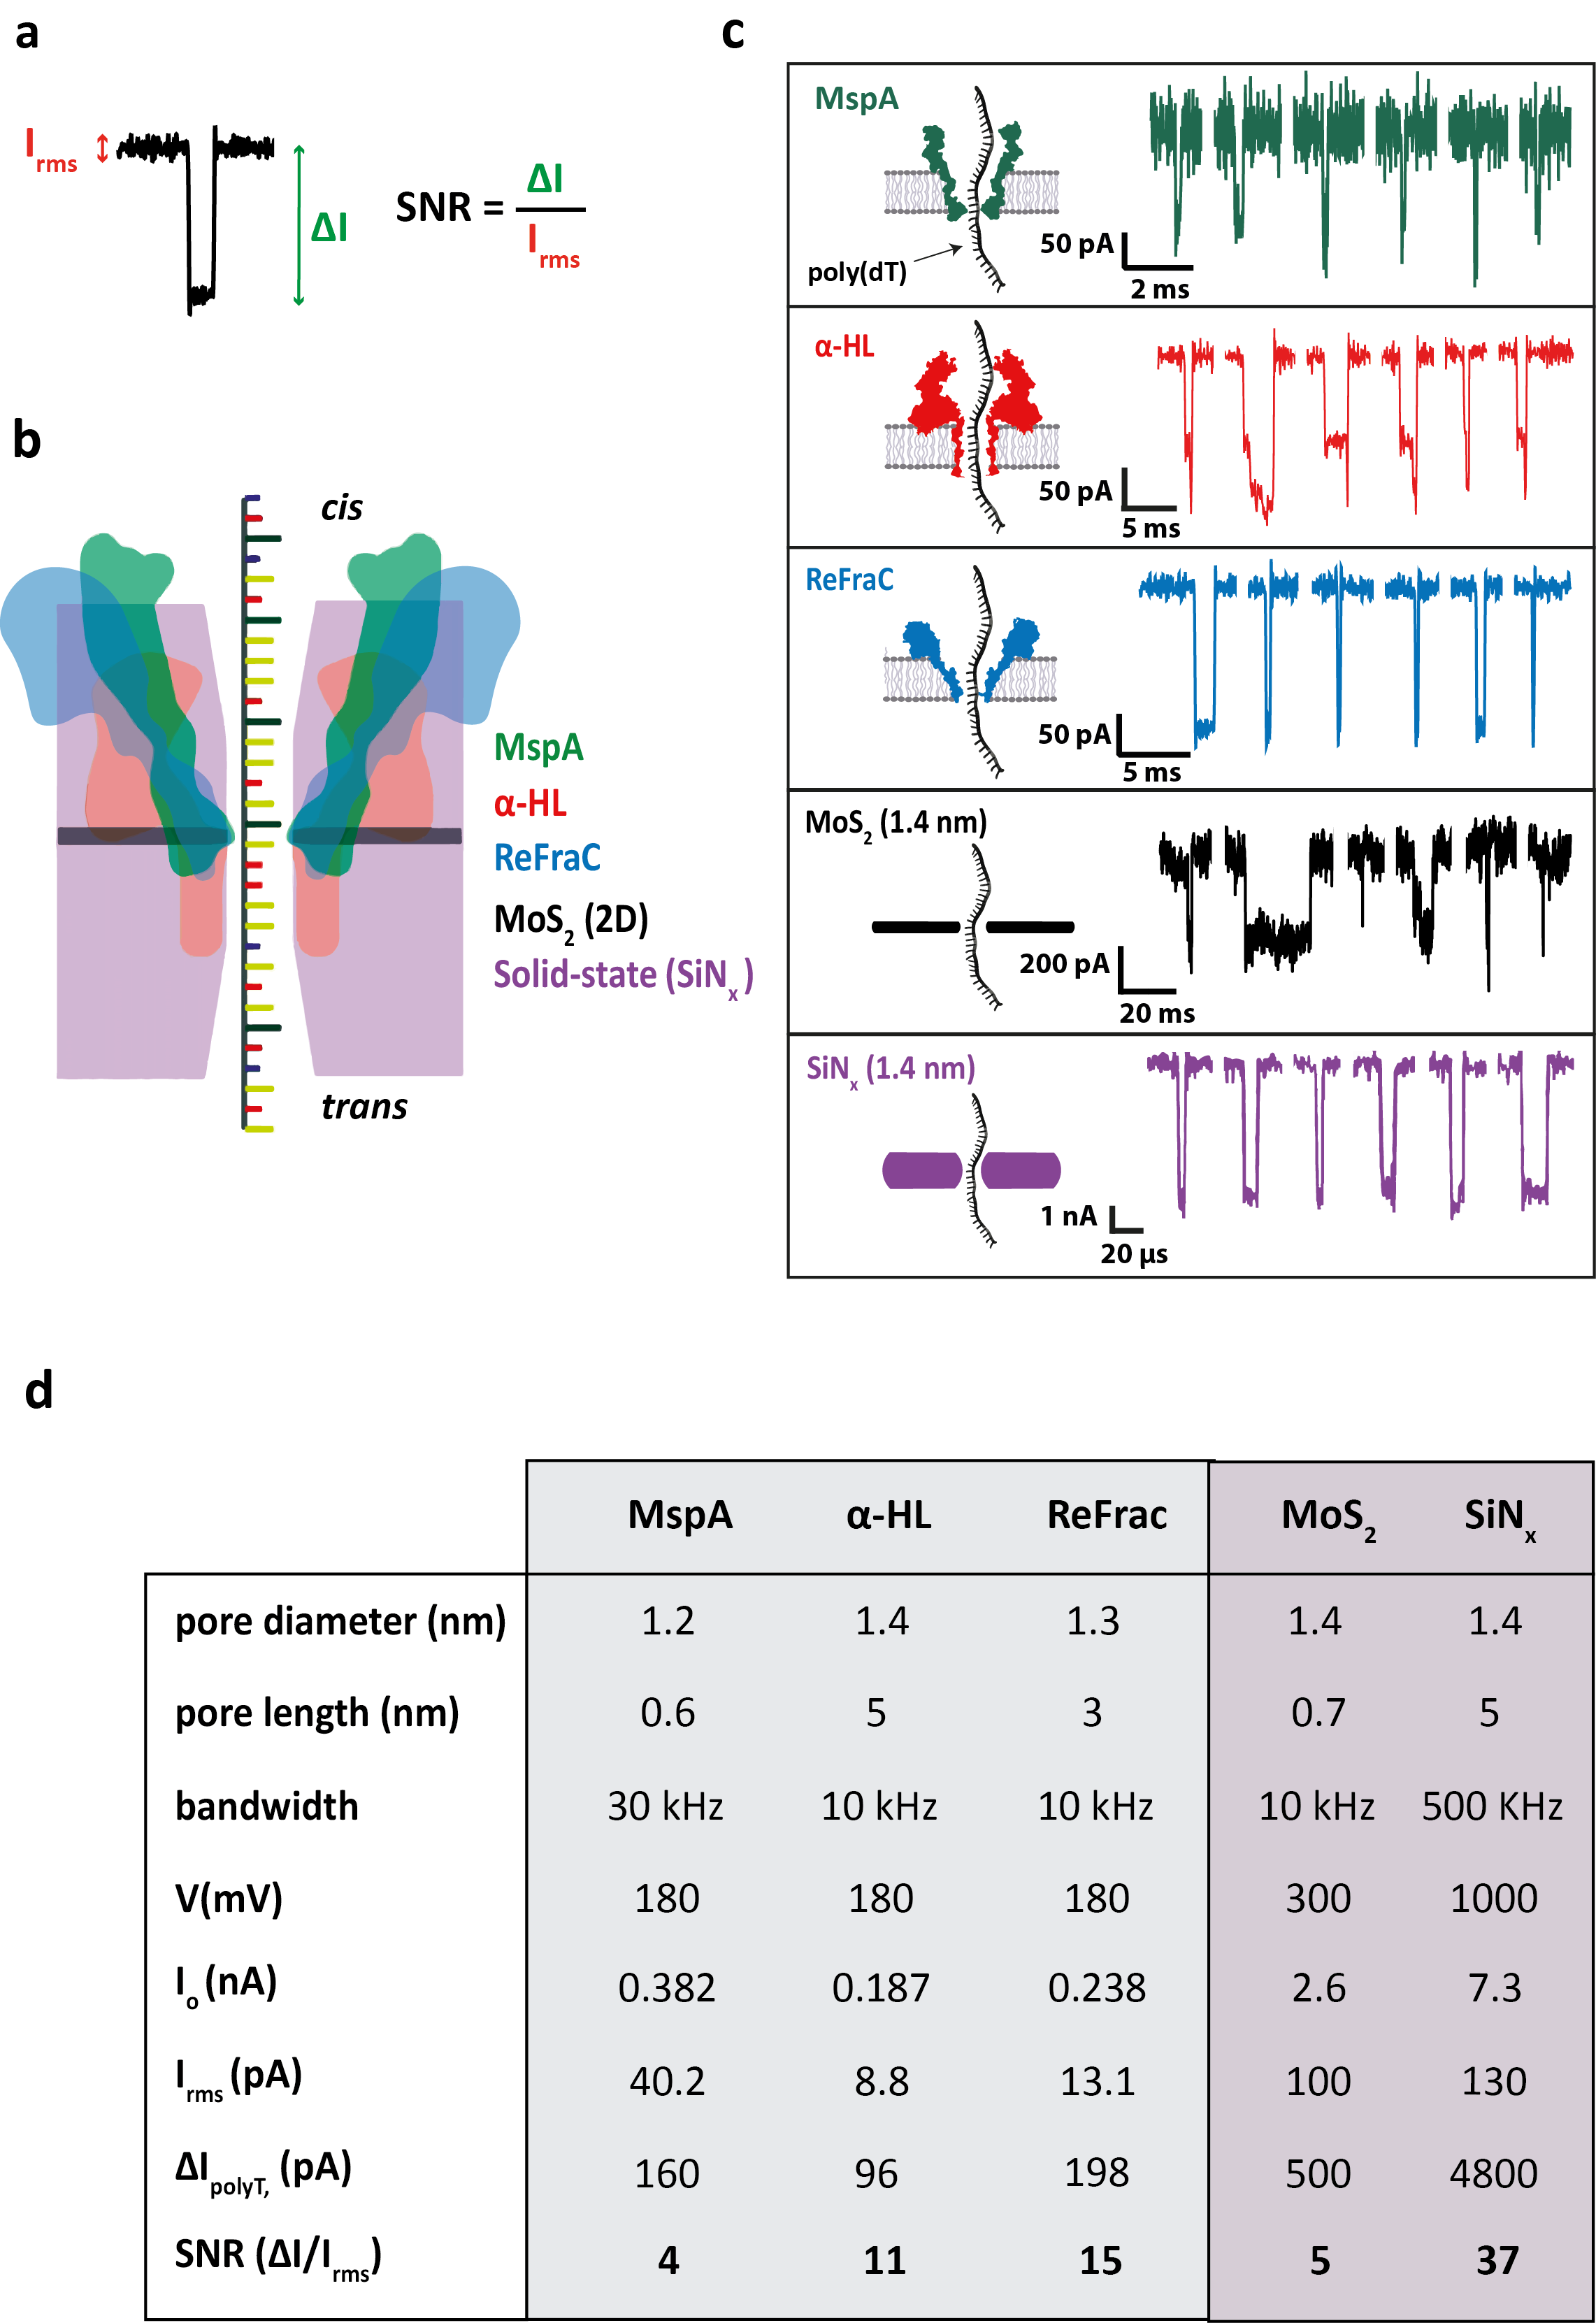
\includegraphics[width=0.7\linewidth]{figures/Figure3.4.png}
	\caption{Detection of DNA homopolymer poly(dT) with protein and solid-state nanopores. (a) Example of a translocation event, illustrating the signal-to-noise ratio. (b) Schematic comparing the relative sizes of MspA (green), $\alpha$-HL (red), ReFraC (blue),  MoS\textsubscript{2} (black), and solid-state SiN\textsubscript{x} (purple). Adapted with permission from Carson, S. \emph{et al.}, 2015.
		%; Wanunu, M. Challenges in DNA Motion Control and Sequence Readout Using Nanopore Devices. Nanotechnology 2015, 26, 74004. Copyright \copyright 2015 IOP Publishing Ltd. 
		(c) Example of translocation events of poly(dT) molecules through MspA \cite{Derrington2010} channel (green), $\alpha$-HL pore (red), ReFraC pore (blue), 1.4 nm MoS\textsubscript{2} pore (black), and 1.4 nm SiN\textsubscript{x} pore (purple, Adapted with permission from Venta, K. \emph{et al.}, 2013)
		%; Shemer, G.; Puster, M.; Rodríguez-Manzo, J. A.; Balan, A.; Rosenstein, J. K.; Shepard, K.; Drndić, M. Differentiation of Short, Single-Stranded DNA Homopolymers in Solid-State Nanopores. ACS Nano 2013, 7, 4629–4636. Copyright \copyright 2013 American Chemical Society
		all in 1 M KCl solution at a transmembrane voltage of 180 mV, 180 mV, 180 mV, 300mV, and 1V, and at a bandwidth of 30 kHz, 10 kHz, 10 kHz, 10 kHz,  and 500 kHz, respectively. Experiments for biological pores were done using an Axopatch 200B amplifier, a teflon-supported lipid membrane ($\sim$50-100 $\mu$m wide; DPhPC lipids), 10-30 kHz bandwidth, 1 M KCl, pH 7.5, and a forward bias voltage of 180 mV, as in Ref.\cite{Butler2008}. The solid-state SiN\textsubscript{x} pore was built on a glass chip and measured with the VC100 high-bandwidth, low-noise voltage-clamp amplifier (Chimera Instruments, New York, NY, USA) which allowed for low-noise measurements at high bandwidth. A broad bandwidth of 500 kHz was required in order to fully resolve the fast translocations ($\sim$22 $\mu$s) \cite{Venta2013} of poly(dT)\textsubscript{30} through the solid-state SiN\textsubscript{x} pore. Notably, the positively charged constriction of ReFraC causes the negatively charged poly(dT)\textsubscript{50} to translocate with much slower ($491\pm 114$ $\mu$s) translocation times compared to MspA ($17.7\pm 1.1$ $\mu$s), which permitted to filter out more high-frequency noise. (d) Comparison of various figures of merit for different nanopore systems under typical experimental conditions. I\textsubscript{0} indicates the open pore ionic current at the applied bias V.}
	\label{fig:fig3.4}
\end{figure}



Nanopore experiments probing the translocation of poly(dT)\textsubscript{50} were carried out in-house using three biological pores, MspA, $\alpha$-HL, and ReFraC. We compared these data to experimental results on two types of solid-state nanopores, SiN\textsubscript{x} \cite{Venta2013} and MoS\textsubscript{2}\cite{Feng2015} that were measured at the same electrolyte conditions. Translocation data of poly(dT)\textsubscript{80} through a 1.4 nm MoS\textsubscript{2} pore were kindly shared by the Radenovic lab \cite{Graf2019}, whereas poly(dT)\textsubscript{30} data for a 1.4 nm SiN\textsubscript{x} pore with $\sim$5 nm length were taken from the literature \cite{Venta2013}. Figure \ref{fig:fig3.4}c shows examples of single-molecule poly(dT) translocations for the 5 pores. A range of SNR values are observed, with, at face value, a better performance for SiN\textsubscript{x} and ReFraC than for MoS\textsubscript{2}, $\alpha$-HL, and MspA. 

Figure \ref{fig:fig3.4}d quantitatively compares the data for the different nanopore systems. 
For the biological nanopores, ReFraC gives the best SNR = 15, while MspA resulted in a much lower SNR of 4. This is mainly due to the faster translocations of poly(dT) through MspA, which required a higher bandwidth (30 kHz), and hence larger noise, in order to resolve the translocation events. Conversely, translocations through the positively charged constriction of ReFraC were significantly slower, thus permitting to employ a lower bandwidth (10 kHz). 

Amongst the solid-state nanopores, SiN\textsubscript{x} showed the best SNR: an impressive value of 37, which was higher than the SNR = 5 obtained for MoS\textsubscript{2}, as well as higher than the values for all biological nanopores. The greater SNR for SiN\textsubscript{x} results from the very high voltage applied (1000 mV vs 300 mV for MoS\textsubscript{2}), producing a particularly large current signal $\Delta$I. The applied voltage for MoS\textsubscript{2} pores was limited by the degradation of the 2D membrane and pore growth under high bias voltages, which typically limited the applied bias to $<400$ mV. 

In biological nanopores the range of bias voltages is limited by the membrane stability, affected by electroporation and rupture around 200-300 mV \cite{Pavlin2008,Tarek2005}. Note furthermore that the SiN\textsubscript{x} nanopore system was operated at a much higher bandwidth (500 kHz vs 10 kHz for MoS\textsubscript{2}), the regime where dielectric and capacitive noise dominate. 

This is advantageous for high-voltage sensing, since these noise sources do not scale with voltage, cf. Eq.\ref{eqn:eq.3.5} and Eq.\ref{eqn:eq.3.6}. As a result, the high bias voltage improves the signal ($\Delta$I) while it does not affect the noise. Lastly, we note that, while MoS\textsubscript{2} has a lower SNR than SiN\textsubscript{x}, it features a better spatial resolution along the molecule, given its 0.7 nm pore length, as compared to the $\sim5$ nm of SiN\textsubscript{x}. 


Finally, it is important to point out that the above comparison was carried out for voltage-driven translocation of DNA through nanopores. A controlled slowdown of the translocation speed can change these numbers dramatically. Indeed, despite the fact that Figure \ref{fig:fig3.4}d shows that the best SNR was obtained for the solid-state SiN\textsubscript{x} nanopores, with values exceeding those of biological nanopores, todays commercialized nanopore-based DNA sequencers employ protein pores to read off DNA bases with (sub)-nucleotide resolution over very long reads \cite{Carter2018,Jain2018}. Using a helicase to slow down ssDNA molecules through MspA, allowed Laszlo \emph{et al.} \cite{Laszlo2016} to use a very low LP filter frequency of $\sim$200 Hz, and fully resolve the step-wise DNA translocation at half-base resolution. By comparing the noise at a 200 Hz bandwidth with the signal obtained for voltage-driven poly(dT) translocations in our experiments, we find an exquisite SNR of $\sim$650 for MspA – two orders of magnitude higher than the SNR = 4 noted above. Applying the same reasoning to $\alpha$-HL and ReFraC increases their SNR to $\sim$270 and $\sim$220, respectively, \emph{i.e.}, somewhat lower values, consistent with their higher low-frequency noise compared to MspA (Fig.\ref{fig:fig3.3}c). Thus, in the context of DNA sequencing, the real game-changer lies in the enzymatic control over the translocation speed by use of an additional motor protein \cite{Manrao2012,Carter2018,Laszlo2016,Manrao2010,Jain2016}. For solid-state nanopores, despite the progresses in slowing down the DNA translocation \cite{Feng2015,Keyser2011,Wanunu2007,Pud2016,Gilboa2015,Yamazaki2018}, time control has so far remained a challenge, and accordingly, DNA sequencing has not yet been realized with such nanopores. Furthermore, mechanical instability of solid-state nanopores over time, which particularly affects smaller pores, should be minimized in order to achieve sufficiently long observation times.


\section{Approaches to overcome noise limitations}


Figure \ref{fig:fig3.5} shows important approaches to lower the ionic current noise in nanopores. We first describe efforts to reduce the low-frequency noise. As protonation noise is the main source of low-frequency noise in biological nanopores, it is advantageous to choose a pH value that is far away from the pK\textsubscript{a} of the ionizable amino acids to attenuate the noise. Another way to reduce it, is to remove charged amino acids near the constriction site, which is expected to yield lower noise levels. Furthermore, increasing the conformational stiffness of biological pores can help to reduce conductance fluctuations associated with channel breathing. 


For solid-state nanopores, the low-frequency 1/f noise can be efficiently suppressed by surface functionalization of the SiN\textsubscript{x} nanopore with a hydrophilic surface layer, such as Al\textsubscript{2}O\textsubscript{3} or SiO\textsubscript{2} \cite{Wang2013,Nilsson2006,Danelon2006,Chen2004}. In principle, any surface treatment that reduces the amount of contaminants and improves hydrophilicity of the pore surface will lower the 1/f noise. Indeed, Tabard-Cossa \emph{et al.} \cite{Tabard-Cossa2007} showed that piranha treatment (30\% H\textsubscript{2}O\textsubscript{2}/H\textsubscript{2}SO\textsubscript{4}, 1:3) substantially reduced the 1/f noise by up to three orders of magnitude. Beamish \emph{et al.} \cite{Beamish2012} demonstrated that cyclic application of high electric fields to the nanopore also suppressed this noise source. Similar to protein pores, work from Wen \emph{et al.} \cite{Wen2017} showed that the 1/f noise could be minimized by choosing a pH that is far from the isoelectric point of the nanopore material ($\sim$5 for Si\textsubscript{3}N\textsubscript{4}) \cite{Kosmulski2002,Firnkes2010}. Nanopores built with 2D materials suffer from pronounced 1/f noise that was found to correlate with the area and thickness of the freestanding 2D-membrane \cite{Montal1972,Sakmann2009}. A decrease of the freestanding area was shown to reduce the 1/f noise, while employing multi-layer membranes was also helpful for obtaining less noise, though that approach is less desirable due to a loss of spatial resolution \cite{Park2016,Heerema2015,Zhang2018}. Use of freestanding 2D-membranes that are directly grown on a SiN\textsubscript{x}-supporting membrane was also shown to lower the 1/f noise for both graphene \cite{Waduge2015a} and MoS\textsubscript{2} \cite{Waduge2015} pores, as compared to transferred 2D-membranes \cite{Merchant2010,Heerema2015}.


The noise at higher frequencies, constituted by dielectric and capacitive noise, has a well-characterized physical origin, namely the thermal voltage noise in conjunction with the loss conductance of the membrane and substrate materials as well as the amplifier input capacitance. Suppression of dielectric noise is generally achieved by minimizing the capacitance $C_{chip}$ and dielectric loss $D$ of the chip, cf. Eq.\ref{eqn:eq.3.5}. To effectively decrease capacitive noise, the total input capacitance $C_{tot}$ needs to be reduced, see Eq.\ref{eqn:eq.3.6} and related discussion. In biological nanopores, the high-frequency noise can be reduced by decreasing the area of the lipid bilayer. Mayer \emph{et al.}\cite{Mayer2003} fabricated teflon holes of only $\sim$25 $\mu$m in diameter with soft lithography using SU-8 resist as master mold, providing 

\begin{figure}[H]
	\centering
	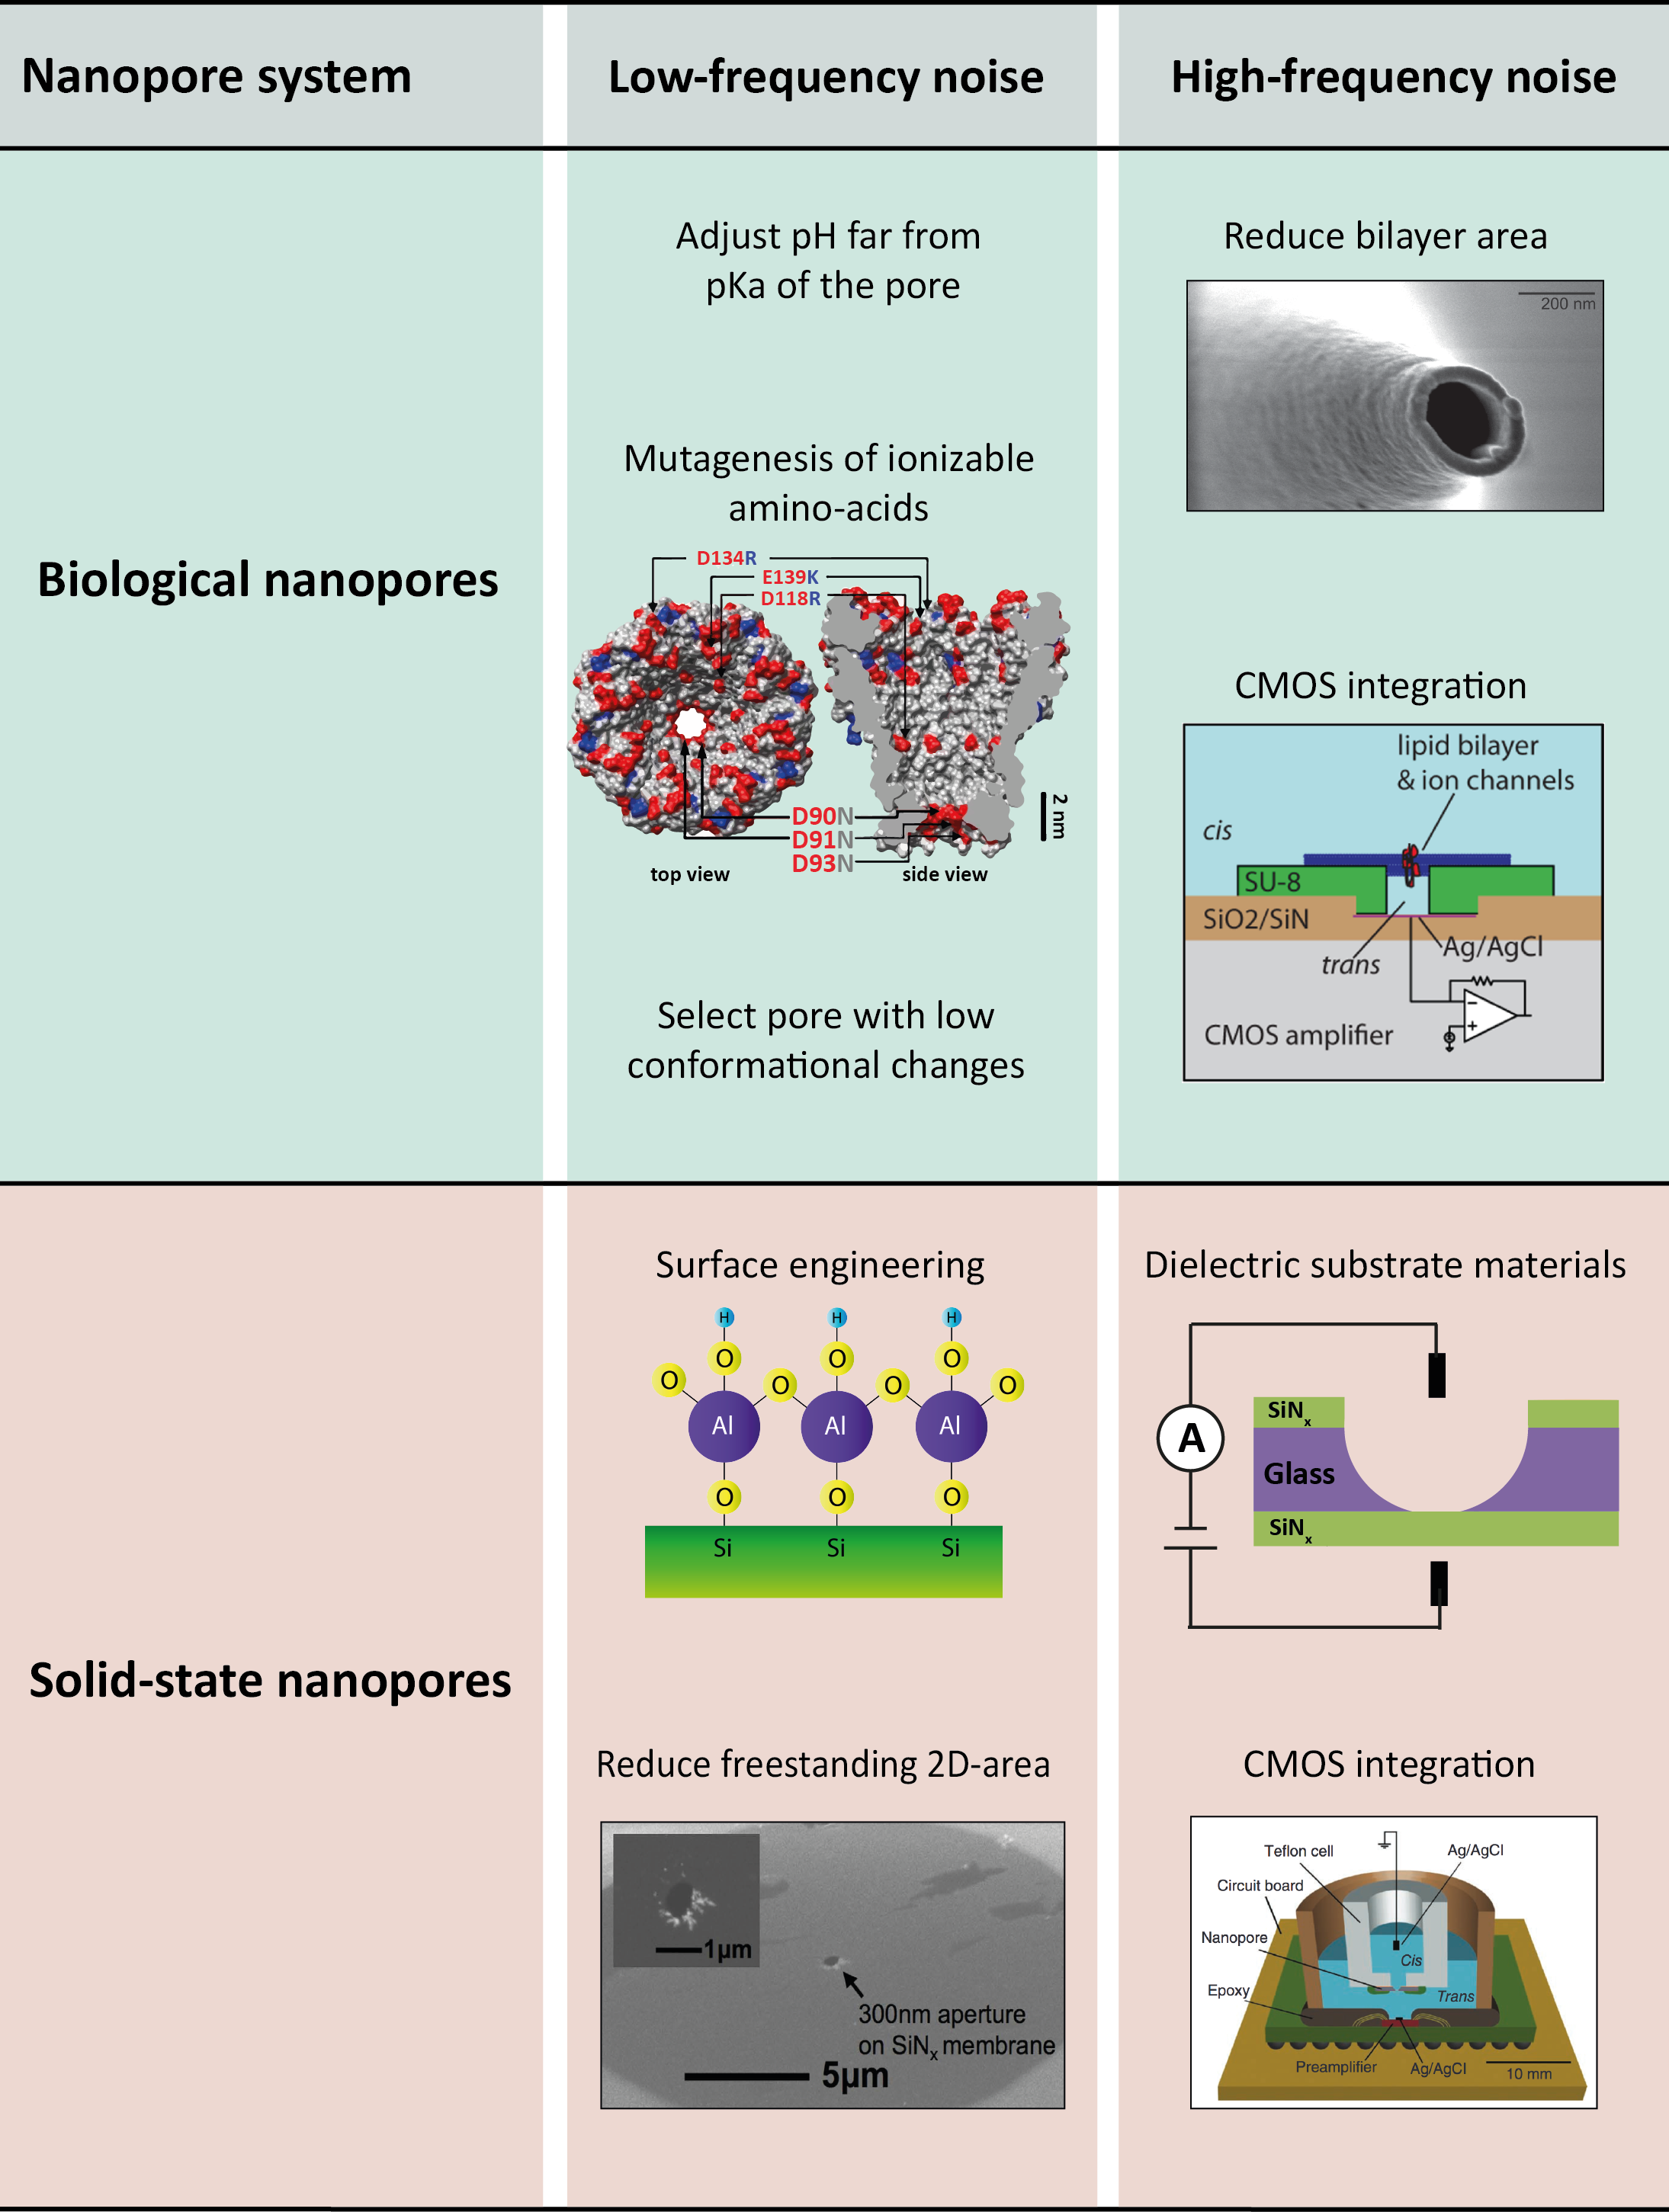
\includegraphics[width=0.8\linewidth]{figures/Figure3.5.png}
	\caption{Approaches to reduce the noise in nanopore systems. For biological nanopores, low-frequency protonation noise can be minimized by adjusting the pH far from pK\textsubscript{a} of the amino acids in the pore constriction, as reported in Ref.\cite{Kasianowicz1993}, or by mutating the ionizable amino acids (Arg, Lys, Asp, Glu) to neutral ones (\emph{e.g.}, Asn), as was done for MspA . Reprinted with permission from Butler, T. Z. \emph{et al.}, 2008 \cite{Butler2008}.
		%; Pavlenok, M.; Derrington, I. M.; Niederweis, M.; Gundlach, J. H. Single-Molecule DNA Detection with an Engineered MspA Protein Nanopore, Proc. Natl. Acad. Sci. 2008, 105, 20647–20652. Copyright \copyright 2008 National Academy of Sciences, U.S.A. 
		Low-frequency 1/f noise instead can only be avoided by selecting a pore that is mechanically stable under an applied bias, \emph{e.g.} MspA or $\alpha$-HL. High-frequency noise can be minimized by reducing the size of the freestanding lipid membrane by, \emph{e.g.}, employing a nanocapillary as a support  (Reprinted with permission from Gornall, J. L. \emph{et al.}, 2011 \cite{Gornall2011})
		%; Mahendran, K. R.; Pambos, O. J.; Steinbock, L. J.; Otto, O.; Chimerel, C.; Winterhalter, M.; Keyser, U. F. Simple Reconstitution of Protein Pores in Nano Lipid Bilayers. Nano Lett. 2011, 11, 3334–3340. Copyright \copyright 2011 American Chemical Society) 
		and by reducing the capacitance of the interconnects by smart CMOS integration (Reprinted with permission from Rosenstein, J. K. \emph{et al.}).
		%; Ramakrishnan, S.; Roseman, J.; Shepard, K. L. Single Ion Channel Recordings with CMOS-Anchored Lipid Membranes. Nano Lett. 2013, 13, 2682–2686. Copyright \copyright 2013 American Chemical Society
		For solid-state nanopores, low-frequency 1/f noise can be reduced by coating the surface with a hydrophilic, homogeneous material, \emph{e.g.} Al\textsubscript{2}O\textsubscript{3}, as reported in Ref.\cite{Chen2004}. For 2D-materials, 1/f noise can be suppressed by lowering the area of the freestanding 2D membrane . Adapted with permission from Balan, A. \emph{et al.}, 2015 \cite{Balan2015}.
		%; Chien, C. C.; Engelke, R.; Drndic, M. Suspended Solid-State Membranes on Glass Chips with Sub 1-pF Capacitance for Biomolecule Sensing Applications. Sci. Rep. 2015, 5, 1–8. Copyright \copyright 2015 Springer Nature. 
		High-frequency noise can be minimized by employing dielectric chip substrate materials, \emph{e.g.} glass (adapted with permission from Balan, A. \emph{et al.}, 2015 \cite{Balan2015},
		%; Chien, C. C.; Engelke, R.; Drndic, M. Suspended Solid-State Membranes on Glass Chips with Sub 1-pF Capacitance for Biomolecule Sensing Applications. Sci. Rep. 2015, 5, 1–8. Copyright \copyright 2015 Springer Nature) 
		or by tight integration of the amplifier and nanopore chip (adapted with permission from Rosenstein, J. K. \emph{et al.}, 2012 \cite{Rosenstein2012}.
		%; Wanunu, M.; Merchant, C. A.; Drndic, M.; Shepard, K. L. Integrated Nanopore Sensing Platform with Sub-Microsecond Temporal Resolution, Nat. Methods 2012, 9, 487–492. Copyright \copyright 2012 Springer Nature)
	}
	\label{fig:fig3.5}
\end{figure}

\noindent a $C_{chip}$ of 10-28 pF. By using a U-shaped teflon patch tube as the support, Akeson and coworkers \cite{Akeson2009,Butler2008} built horizontal bilayers $<20$ $\mu$m in diameter. Lipid bilayers with a comparable size were also created with the droplet-interface-bilayer (DIB) technique \cite{Bayley2008}. Kitta \emph{et al.} \cite{Kitta2009} reported on the fabrication of yet smaller bilayers, with sizes down to 2-3 $\mu$m in diameter, by using a heated tungsten tip to create a microhole across the teflon film. 
Similarly sized 1-3 $\mu$m bilayers can be obtained by inserting protein pores into GUVs (Giant Unilamellar Vescicles) and using patch-clamp pipets to measure the conductance of the pores \cite{Criado1987,Riquelme1990}. More recently, Gornall \emph{et al.} \cite{Gornall2011} showed that borosilicate glass nanopipets with diameters as low as 230 nm could be fabricated and used for current recordings on an OmpF protein channel. Hartel \emph{et al.} \cite{Hartel2018} achieved high-bandwidth ($>500$ kHz) recordings with biological pores with CMOS-suspended (Complementary Metal-Oxide-Semiconductor) membranes that were built directly over a $\sim$30 $\mu$m well on top of a CMOS-amplifier chip. This offered a reduction of the total input capacitance $C_{tot}$ to $<4$ pF and provided a bandwidth as high as 1 MHz and a SNR $>8$  at 500 kHz, for detecting the gating of a RyR1 pore (type 1 ryanodine receptor) \cite{Hartel2018}. Combined with extended $\beta$ distribution data analysis \cite{Schroeder2015} (which exploits the characteristics of the excess current noise to reconstruct the true current signal), it was possible to achieve a time resolution of 35 ns \cite{Hartel2018}. 


For reducing the high-frequency noise in SiN\textsubscript{x} solid-state nanopores, an established method, first reported by Tabard-Cossa \emph{et al.} \cite{Tabard-Cossa2007}, is to lower $C_{chip}$ by coating the area of the chip around the pore with a dielectric, e.g. PDMS, thereby providing additional thickness to the chip membrane surrounding the pore and thus a low series capacitance. Similarly, a substantial reduction of $C_{chip}$ was achieved by employing a dielectric, \emph{e.g.} amorphous glass \cite{Balan2014,Balan2015} or Pyrex \cite{Park2016,Pitchford2015} as substrate material instead of the commonly used crystalline silicon which is intrinsically conductive. In work by Balan \emph{et al.}, \cite{Balan2015} glass chips were shown to reduce $C_{chip}$ to $<1$ pF, compared to $>300$ pF for standard silicon chips \cite{Smeets2008}. Similarly to biological nanopores, the highest working bandwidths were so far achieved by integrating a low $C_{chip}$ nanopore device with an on-chip CMOS-amplifier \cite{Rosenstein2012,Shekar2016}, which lowered the total input capacitance to $C_{tot}\approx 4$ pF. In this way, ssDNA molecules were recorded using ultrathin ($<4$ nm) sub-2 nm pores yielding a SNR$>10$ at 5 MHz \cite{Shekar2016}. In 2D nanopores, the high-frequency noise can be addressed in similar ways to SiN\textsubscript{x} pores. The use of glass as substrate material, combined with a small $\sim$300 nm freestanding 2D-membrane of graphene or MoS\textsubscript{2}, resulted in a $C_{chip}<2$ pF \cite{Balan2015}. 


\section{Conclusion}


In this paper, we illustrated the main sources of noise affecting various nanopore systems, with a particular emphasis on comparing biological and solid-state nanopores, and we discussed practical approaches to lower the noise. We compared the SNR of poly(dT) translocations through a representative set of biological and solid-state pores, and found that silicon nitride nanopores gave the highest SNR. This can be attributed to the higher currents (\emph{i.e.} larger signals) that solid-state systems offer, and to the relatively low high-frequency noise. Despite these good noise characteristics, prominent applications such as DNA or protein sequencing have so far remained out of reach for solid-state nanopores, because the fast translocation speed provides only a short observation time per single molecule. There are two ways to improve this: one can either shift the sampling rate into even higher frequencies ($\gg$ MHz), or alternatively slow down the translocation of the molecule. The latter strategy has led to the successful commercialization of DNA sequencers based on protein nanopores that are coupled with an enzymatic stepping motor. In our comparison, we found that the SNR of MspA increased $>160$-fold by such speed control, mainly due to the decoupling of the signal from the high-frequency noise. Additionally, the motor protein provides a ratcheting mechanism that translocates the substrate with a constant discrete step size. Since the sensing region of the pore is typically larger than the individual monomer size (nucleotide or amino-acid), such a mechanism is indispensable to reproducibly resolve and identify the sequence. Future improvements of the solid-state nanopore system could thus be directed towards either a further increase of the temporal resolution, e.g. by reducing even more the overall parasitic capacitances, or by creating an efficient slowdown mechanism, similar to biological nanopores. In general, the understanding of noise sources, associated timescales, and techniques to lower the noise at both low and high frequencies are greatly beneficial to maximize the sensitivity of nanopore detection and thereby extend the range of its applications.





\references{chapter-3/chapter-3}
